%----------------------------------------------------------------------------------------
%	Introduction
%----------------------------------------------------------------------------------------



\chapter{Introduction}\label{chap:intro}
\fancyhead[L]{\textit{Chapter 1. Introduction}}


{\textit{``To develop a complete mind: Study the science of art; Study the art of science. Learn how to see. Realize that everything connects to everything else."}}

\rightline{--- Leonardo Da Vinci}




\section{How connected are real world networks?} \label{sec:work}

Stanley Milgram in his classic paper, \emph{The Small-World Problem} \cite{milgram}, put forth the notion of transitive dependency among people in a social network. He states that when a person, named Bob, is connected by a series of links to another person, called Alice, there are, on average, five intermediate people between Bob and Alice. 
Brown and Reingen \cite{brown} studied real networks and found the importance of stronger and weaker links associated with recommendation systems. Stronger links are seen as a measure of reliability for a certain recommendation, whereas weaker links are associated with the traversal of information from one cluster to another playing an important role in the networking ecosystem.


Social networking sites have seen a significant boom in the past two decades. These sites play a crucial role in spreading new ideas or innovations through its fundamental network structure consisting of individuals and their relationship with other individuals. Major networking sites with over a hundred million active users include \emph{Facebook, Twitter, Instagram}, etc. In other words, \emph{social networks} are a collection of \emph{entities} which form \emph{relationships} with other entities participating in the same network. 


Due to the increase of information propagation in the networking sites, networks have become increasingly complex. Researchers have been trying to decode the properties and patterns exhibited by such massive networks. \emph{Social Network Analysis (SNA)} has emerged as the study of social networks using \emph{collaboration graphs}, in which the entities are modelled by the nodes of a graph and the relationship between the entities are modelled by a set of edges. Formally, a \emph{Social Graph} $G = (V, E)$ is a directed graph (sometimes undirected), where \emph{V} is the set of nodes representing the entities of the network, and $E$ is the set of edges  representing the relationship existing between those entities. SNA is the field of study at the intersection between \emph{Graph Theory, Networking} and \emph{Sociology}.



\section{Application of social networks: Viral Marketing}

\emph{Marketing} is the promotion of a product by a company to its customer base. It takes into account the \emph{word-of-mouth} effect, i.e., a customer who has used the products, can recommend it to her friends. \emph{Viral Marketing (VM)} supports the same theory, and uses social networks as a platform for recommendations. The method follows the principle of contiguous viruses: if the flu infects one person, any person who comes in contact with the infected person also catches the flu with high probability.

In social networks, the company distributes some free or discounted products to specific individuals who are capable of marketing it. These individuals may recommend it to their neighbours after using it, who in turn might recommend it to their neighbours, and so on, following an iterative diffusion process. The direct analogy to this is \emph{Influencer Marketing}. Influencers are those particular individuals in the network, who have a significant number of followers in a specific niche, and can affect the decisions of the people following her. Companies who want to launch new products in the market generally offer their products to the influencers, particularly to those who are closer to the specific customer base for selling the considered products. 

Krackhardt et al.~\cite{Iacobucci2014} states that a marketer can leverage her sales profit by knowing the topology of the underlying social network. They also introduced the concept of distributing free products to the influencers. Domingos and Richardson~\cite{Domingos2001,Richardson2002} introduce some models of viral marketing, and raise the following algorithmic question: \textit{in a vast connected network, if a seller markets a product, how should they choose a set of influential buyers (nodes) who can reach out to (influence) as many nodes as possible to buy that product?} Indeed, the number of such buyers are directly proportional to the seller's profit. Kempe et al.~\cite{Kempe2003,kempe05,Kempe2015}, in their seminal works, presented VM as a discrete optimization problem, and called it the \emph{influence maximization (IM)} problem, discussed in details in the upcoming sections and chapters.      

\section{From viral marketing towards maximizing influence in networks}

The IM problem as described by Kempe et al.~\cite{Kempe2003} is an one-shot task: given a static social network $G$, a diffusion model with given parameters, select the seed set $S$, and with only one propagation pass through the entire network, $S$ activates $k$ nodes, with the expectation of maximizing the number of active nodes in the network. 


The utility function, $f$, which needs to be maximized is shown to be submodular ($f$ satisfies the ``diminishing returns" property) and  monotone (number of active nodes either increase or remain the same). Since the problem is NP-hard by nature (shown by reduction through \textit{Set Cover Problem}), approximation algorithms needs to be used. From the results of Nemhauser et al.~\cite{Company1978, nemhauser}, Kempe et al.~\cite{Kempe2003} showed that the results obtained from a simple greedy algorithm will reach at least $(1-1/e)$ of the optimal solution.


\subsection*{Independent Cascade (IC) Model}

Goldenberg et al.~\cite{J.2001}, Goldberg and Liu \cite{Goldberg2013} used the concept of \emph{Cellular Automata} as a framework to model the diffusion of information in the network. The \emph{Independent Cascade(IC)} model, named by Kempe et al.~\cite{Kempe2003} models the dynamics of the viral marketing scenario and draws inspiration from the field of interacting particle systems. Initially, the diffusion model starts with a set of active nodes $S$ such that $|S| \leq k$. Each edge $e=(u,v)\in E$, has an influence probability $p_{uv}$ attached to it, so that node $u$ will activate node $v$ with a probability $p_{uv}$, independently from the other nodes. 

With the above parameters as input to the system, the diffusion process unravels in several time steps. At time step $t$, if node $u$ is active, it is given a single opportunity to activate its neighbour $v$ with probability $p_{uv}$. If node $v$ becomes active at time step $t$, it will further attempt to activate its neighbours at time step $t+1$ according to the influence probability. The process iteratively continues and comes to a halt when there are no more activations. Since the diffusion process spreads in a cascading manner, and each activation is independent from the other, the model is named as the independent cascade model.


\paragraph*{Linear Threshold (LT).} Differently from the IC model, where each activation is independent from each other, the LT model follows a more complex contagion process. Each node $v$ is  associated with a threshold value $\theta_v$, and to activate $v$, the probability associated with the  active edges from $v$'s neighbours need to cross the threshold $\theta_v$. This model is not in the scope of the thesis except for the experimental part in Chapter \ref{chap:background}. However, in Chapter \ref{chap:lit}, Section \ref{sec:lt} we will discuss the technical part of the LT model. 

\subsection*{Adaptive Influence Maximization}

In the \emph{Adaptive Influence Maximization (AIM)} \cite{Golovin2011}, we consider the adaptive version of the IC model. An adaptive policy $\pi$ is a function associating the {\em network state} with a new node that should be added to the seed set $S$, where the network state is what a policy observes at each time. The function $f$ that we want to maximize in expectation is the number of nodes that are reached by the spread of information.

The AIM problem wants to find a policy with a seed-set maximizing the expected value of $f$ (according to the probability distribution of the realizations), where the cardinality of the seed set must be at most $k$. The seed nodes are selected in multiple time steps, based on the observations or feedback obtained from the previous steps. The quality of seed nodes selected under the adaptive setting is better and also the influence generated is further improved because of the feedback provided by the network.




\subsection*{Feedback models}

There are two commonly used feedback models: \textit{full adoption} and \textit{myopic}. A full adoption feedback model records the entire spread generated by a seed node. The adaptive policy $\pi$ observes this feedback and then decides on the selection of the next seed node. As mentioned before, the underlying diffusion model considered in this thesis is the independent cascade model, which is adaptive submodular and monotone for the full adoption feedback~\cite{Golovin2011a}. Golovin and Krause~\cite{Golovin2011a} exploited the desired adaptive submodularity property of the objective function $f$, and applied the results from Nemhauser et al.~\cite{nemhauser,Company1978} to show that the solution provided by an adaptive greedy policy is at least $(1-1/e)$ of the optimal adaptive policy.

The myopic feedback model observes the current state of a seed node's immediate neighbours only. This model is shown to be adaptive non-submodular by nature in \cite{Golovin2011}. In order to evaluate the performance of this model, we need to recover the adaptive submodularity via an artificial diffusion model, which gives a seed node multiple chances to activate its neighbours \cite{Chen2019, DAngeloPV21}. The feedback models will be discussed later at length in Section \ref{feedback}.

\subsection*{Adaptivity Gap}

Another important term coined by Golovin and Krause~\cite{Golovin2011a} is the \emph{Adaptivity Gap (AG)}. The AG quantifies how well does an optimal non-adaptive policy, that is a policy in which all the edges should be selected at beginning, without observing the realization, perform when compared to an optimal adaptive policy. To measure the efficiency of a non-adaptive greedy algorithm, we can multiply the adaptivity gap with the approximation factor to compare the performance ratio of the algorithm with the optimal adaptive policy.



\section{Necessity to bound the Adaptivity Gap} \label{sec:ag}

Due to the feedback received after every round of seed selection, the efficiency in terms of time reduces for an adaptive policy. However, a non-adaptive policy is a straightforward simple process, and the overhead in time is negligible compared to the adaptive policies. 
Also, a non-adaptive algorithm is much simpler to design since the seed selection takes place in the beginning of the diffusion process, and we do not keep track of the nodes that are activated at each time step. 

 
\begin{figure}
\centering
    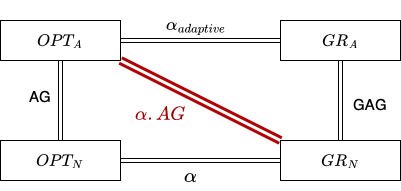
\includegraphics[width=0.7\linewidth]{GSSI_thesisProposal/figures/AG.png}
    \caption{Connection between optimal and greedy policies.}
\label{fig:ag}
\end{figure}

The adaptivity gap gives us the ratio to check how efficient the seed set selected by the optimal non-adaptive policy is compared to the adaptive optimal over different graph classes. A tighter bound is preferred, but the main challenge is to find an upper bound that is closer to 1, which will indicate that there exists an optimal non-adaptive policy that is as efficient as the optimal adaptive policy for that graph class. 
The thesis tries to find and then improve on these upper bounds on the different graph classes using newer techniques and by studying the ones that are used in the past. 

In Section \ref{exp} we will encounter the efficiency of the adaptive greedy algorithm based on the memory consumption. With a faster best estimate, the non-adaptive greedy policy tends to consume a huge part of the memory as the size of the graph grows, hence asking for better memory management. A non-adaptive greedy algorithm is generally preferred over an adaptive one due to the above stated reasons, and hence a measure is needed to calculate the efficiency of such algorithms. Another measure called the \emph{greedy adaptivity gap (GAG)} \cite{Chen2019a}, which measures the generated spread  between the greedy adaptive algorithm and the greedy non-adaptive algorithm, helps us to navigate through the performance efficiency of a non-adaptive greedy algorithm over a adaptive greedy one. Figure \ref{fig:ag} depicts the ratio between the optimals and the greedy algorithms (refer to table \ref{sec:not} for the notations used in the figure). The diagonal red line is the most important factor to bound, since it directly estimates by how much an optimal adaptive strategy outperforms a non-adaptive greedy algorithm, and helps us to design better algorithms by having an optimal measure in mind. 


\section{Contributions} \label{sec:cont}

\begin{enumerate}


    \item  \textit{Gianlorenzo D’Angelo, Debashmita Poddar, and Cosimo Vinci ``Better bounds on the adaptivity gap of influence maximization under full-adoption feedback", Thirty-Fifth AAAI Conference on Artificial Intelligence, AAAI, 2021.}

    The extended version of the above paper is accepted at the \textit{Artificial Intelligence Journal (AIJ)} \cite{AIJ}.

\paragraph{Full-adoption feedback.}


 

Chapter \ref{chap:background} is mainly related to the results obtained in the aforementioned paper (that is, \cite{DAngelo}), in which we conduct an extensive study on the full adaption feedback model under IC. 
First, we tackle the in-arborescences, which were already studied by \cite{Chen2019} in the adaptive setting. Chen and Peng \cite{Chen2019} derived an upper bound on adaptivity gaps using Poisson process and multi-linear extensions. We bypass those techniques and give a simpler and quicker solution to connect the non-adaptive and adaptive optimals. Eliminating the techniques used by \cite{Chen2019} and building the proof on the marginals related to the hybrid non-adaptive policy reduces the upper bound on adaptivity gap for the in-arborescences from 3.16 to 2.31 (Section \ref{sec_inarb}).

We further exploit our technique, to arrive at the first ever sub-linear upper bound on general graphs. To the best of our knowledge, this is the first and only bound known for general graphs with this setting. We show that under the Independent Cascade model with a full adoption feedback, the adaptivity gap of general graphs is $\lceil n^{1/3}\rceil$, where $n$ is the number of nodes in the graph (Section \ref{sec_gen}).

Next, we derive results on more specific graphs such as the $\alpha$-bounded graphs that includes several undirected graph topologies like a star, cycle, clique (with more than 3 nodes), etc. The $\alpha$-bounded graphs are undirected graphs where for nodes more than degree 2, their degree summation is at most $\alpha$. We show that the adaptivity gap for such bounded graphs is $\sqrt{\alpha}+O(1)$ and for 0-bounded graphs we get 3.16 as the upper bound (Section \ref{sec_alpha}).

We also address a very interesting class of graphs called the $(\beta,\gamma)$-bounded-activation graphs which denotes a cluster of graphs where the nodes that have at most $\gamma$ neighbours have $\beta$ influence in expectation. For $k \geq 2$, the adaptivity gap for such influence graphs is $\sqrt{\beta}+\frac{1}{1-\gamma}$ (Section \ref{sec:beta}).

The chapter is concluded by a series of experiments (Section \ref{exp}) on a bunch of well known networks (generated), that simulate the network (Erdős-Rényi,Watts-Strogatz and Barabási-Albert) and a real world Facebook network. This part includes new results that have not yet been published, and shows how a state-of-the-art non-adaptive greedy algorithm ($TIM^+$) performs when compared to its adaptive counterpart, which has the same underlying code as the non-adaptive greedy. We observe that the greedy adaptivity gap, which is the ratio between the adaptive greedy spread and the non-adaptive greedy, is closer to one for almost all the different network settings. This directly implies that the greedy non-adaptive algorithm ($TIM^+)$ used here, has an efficiency rate close to that of a greedy adaptive algorithm.




 
 \item  \textit{Gianlorenzo D’Angelo, Debashmita Poddar, and Cosimo Vinci ``Improved approximation factor for adaptive influence maximization via simple greedy strategies", 48th International Colloquium on Automata, Languages, and Programming, ICALP, 2021.}



\paragraph{Myopic feedback.} 


Chapter \ref{chap:sota} represents the aforementioned work (that is, \cite{DAngeloPV21}) which improves on \cite{Chen2019a}. The main difficulty faced with the myopic model is the lack of adaptive submodularity. This drawback makes the model non-trivial to analyze and hence we resort to an artificial model called the 2-level diffusion model. We use a similar concept introduced by \cite{Chen2019a}, where the seed node gets multiple chances to activate its neighbours. However, instead of using random walks on optimal decision trees and multilinear extension like in \cite{Chen2019a}, we directly analyze the non-adaptive greedy algorithm and relate it to an optimal adaptive solution which in turn improves the upper bound on the adaptivity gap from 4 to 3.164.

This flexibility of not passing through the adaptivity gap, gives us a more direct and improved approximation factor for both the non-adaptive greedy algorithm and the adaptive greedy. For achieving the approximation ratio for non-adaptive greedy algorithm we resort to a randomized non-adaptive policy to relate the expected spread of the non-adaptive greedy with the adaptive policy and arrive at 0.316, which is an improvement from 0.158 (Section \ref{sec_nag}).

The approximation factor for the adaptive greedy algorithm is found in a similar fashion by introducing the strong 2-level diffusion model and a strong 2-level hybrid policy. The difference with the above mentioned policy lies in the fact that the strong hybrid policy is conditioned by the partial realisations, which is not the case in the simple hybrid adaptive policy. The approximation factor is bounded by 0.393 for the adaptive greedy (Section \ref{ad-sec}).
\end{enumerate}

\section {Organization of the Thesis} \label{sec:org}
This thesis approaches on bounding the adaptivity gap using different techniques, and elucidates on the feedback models with different graph classes. The underlying diffusion model considered here is the independent cascade model and a part of the experiment is conducted on linear threshold.

\begin{itemize}

    \item \textit{Chapter \ref{chap:intro}} gives a general overview of the contents of this thesis and gives a high-level introduction on the topics that will be tackled here. A table of notations is provided to ease the access of all the symbols that will be used throughout the thesis.
    
    \item \textit{Chapter \ref{chap:lit}} carries out an in-depth analysis of the IM problem with the different diffusion models. The chapter continues to provide further details on the AIM problem, an exhaustive analysis of the feedback models and their adaptivity gaps. Furthermore, the chapter navigates through the related state-of-the-art research that has been conducted in this field. 
    
    \item \textit{Chapter \ref{chap:background}} studies the full-adoption feedback under the IC model with different graph classes (in-arborescences, general graphs, $\alpha$-bounded-degree graphs, $(\beta,\gamma)$-bounded-activation graphs). The chapter contains new techniques and the corresponding results on the upper bound of the AG related to the above mentioned graphs. The last part of the chapter deals with experiments which is important to uncover the efficiency of the greedy algorithms with different networks and parameters, giving us a further insight of the complexity to bound both the adaptivity gap and the greedy adaptivity gap.
    
    \item \textit{Chapter \ref{chap:sota}} contains the results related to the infamous adaptive non-submodular myopic feedback model with IC and explores a new way of reducing the upper bound on AG. The chapter also explores the greedy algorithms to achieve better approximations on the adaptive greedy and the non-adaptive greedy algorithms.
    
    \item \textit{Chapter \ref{chap:proposal}} concludes the thesis by summarizing the main results obtained during the PhD. There is a dedicated section related to some application of the graph classes and feedback models studied in the thesis to motivate further research on this topic. Lastly, we discuss the open problems that can be tackled in the future by referring to the works conducted in this PhD thesis. 
    \end{itemize}

\pagebreak

\section{Table of Notations} \label{sec:not}

    \begin{table} [ht]
    \centering
    \caption{Table of Notations}
    \begin{adjustbox}{width=1\textwidth}
    \begin{tabular}{ | c | c | }
    \hline
    \textbf{Symbol}& \textbf{Meaning} \\ [1ex]
     \hline
     \hline
    $[k]_h$&  $\{h, h+1,....,k\}$; $h \leq k$\\ [1ex] \hline
    $G(V,E)$& A graph with $V$ as the set of vertices and $E$ as the set of edges.  \\[1ex]  \hline
    $(u,v)$& An edge between nodes $u$ and $v$: if directed, $u$ has an outgoing edge to $v$.  \\[1ex]  \hline
    $p(uv)$ & Activation probability associated to the edge $(u,v) \in E$  \\[1ex]  \hline
    $n$& Total number of nodes in the graph ; $|V|:=n$\\ [1ex]  \hline
    $m$& Total number of edges in the graph \\ [1ex]  \hline
    $k$& Total number of selected seed nodes\\[1ex] \hline
    $i$ or $j$& Generic nodes\\[1ex] \hline
    $S$& Set of selected seed nodes; $S \subseteq V$, $|S| \leq k$ \\[1ex] \hline
    $A_t$& Activated nodes at step $t$. \\[1ex] \hline
    $L(V,L(E))$& A random graph $L$ made from $G$ and called a live edge graph; $L(E) \subseteq E$\\[1ex] \hline
    $R(S,L)$& Set of nodes activated by $S$ in $L$.\\[1ex] \hline
    $\sigma(S)$& Expected influence spread of $S$; $\mathbb{E}_L[|R(S,L)|]$\\[1ex] \hline
    $\phi_L$& Realization associated with $L$, $\phi_L : V \rightarrow 2^V$\\[1ex] \hline
    $\psi(v)$& Partial realization, set of nodes activated by $v$; $\psi : V \rightarrow 2^S$\\[1ex] \hline
    $dom(\psi)$& Domain of $\psi$\\[1ex] \hline
    $R(\psi)$& Set of nodes activated by $dom(\psi)$\\[1ex] \hline
    $f(\psi)$& Number of nodes activated by  $dom(\psi)$; $f(\psi) = |R(\psi)|$\\[1ex] \hline
    $\psi'$& Sub-realization of $\psi$ if $dom(\psi') \subseteq dom(\psi)$\\[1ex] \hline
    $\pi$& Adaptive policy \\[1ex] \hline
    $\pi(\psi)$& Seed node returned by $\pi$ after taking $\psi$ as an input\\[1ex] \hline
    $\sigma(\pi)$& Expected influence spread of $\pi$\\[1ex] \hline
    $\pi^*$& Optimal adaptive policy\\[1ex] \hline
    $OPT_N(G,k)$& Optimal solution of the non-adaptive problem\\[1ex] \hline
    $OPT_A(G,k)$& Optimal solution of the adaptive problem\\[1ex] \hline
    $AG(G,k)$& Adaptivity Gap\\[1ex] \hline
    $T(V,F)$& A rooted tree\\[1ex] \hline
    $\Delta(i|\psi)$& Expected marginal gain of $i$ when it is added to $\psi$\\[1ex] \hline
    $\rho$& Random variable; $\mathbb{P}[\rho=i]=x_i/k$\\[1ex] \hline
    $\partial(R(\psi))$& Set of boundary nodes of $R(\psi)$; Lemma \ref{lemm2} of Chapter \ref{chap:background}.\\[1ex] \hline
    $deg_v(G)$& Degree of node $v$ in $G$\\[1ex] \hline
    \end{tabular}
    \end{adjustbox}
    \end{table}
    
    
    
    
    \begin{table} [ht]
    \centering
    \begin{adjustbox}{width=1\textwidth}
    \begin{tabular}{ | c | c | }
    \hline
    \textbf{Symbol}& \textbf{Meaning} \\ [1ex]
     \hline
     \hline
     $\mathcal{T}$& Rooted binary decision tree \\[1ex] \hline
     $d$& Depth of the cascade in the partial feedback model \\[1ex] \hline
     $\tau$& Threshold value related to the RIS algorithm \\[1ex] \hline
     $\mathcal{R}$& Set of reverse reachable (RR) sets in RIS  \\[1ex] \hline
     $r$& Number of rounds \\[1ex] \hline
     $\alpha$& Approximation factor of a greedy algorithm (not the $\alpha$ in Chapter \ref{chap:background}) \\[1ex] \hline
     $X$& Random variable \\[1ex] \hline
    $N(u)$& Set of out-neighbors of node u; Section \ref{sec:beta} Chapter \ref{chap:background}\\[1ex] \hline
    $\beta$& $\beta > 0$ is an integer; Section \ref{sec:beta} Chapter \ref{chap:background}\\[1ex] \hline
    $\hat{S}$& Set of nodes such that $|\hat{S}| \leq \beta$; Section \ref{sec:beta} Chapter \ref{chap:background}\\[1ex] \hline  
    $\gamma$& $\gamma \in [0,1)$ such that $\gamma \geq \sum_{v\in N(u)}p_{u,v}$; Section \ref{sec:beta} Chapter \ref{chap:background}\\[1ex] \hline
    $b$& Number of nodes in each batch\\[1ex] \hline
    $G_u$& Residual graph\\[1ex] \hline
    $Rand_t$& Randomized non-adaptive policy\\[1ex] \hline
    $\xi$& Partial state; Chapter \ref{chap:sota}\\[1ex] \hline
    $\bm{\hat{L}}$& A live edge graph distributed as $\bm{L}$, but independent from it\\[1ex] \hline
    $\bm{L^2}(S)$& 2-level-live edge graph with a seed set $S$\\[1ex] \hline
    $\sigma^2_{\bm{L},\bm{\hat{L}}}(S)$& The influence spread of $S$ in $\bm{L^2}(S)$\\[1ex] \hline
    $\sigma^2(S)$& Expected influence spread of S under the 2-level diffusion model\\[1ex] \hline
    $Hyb_t$& Hybrid adaptive policy; Chapter \ref{chap:sota}\\[1ex] \hline
    $\hat{\Phi}_\pi$& Random realization returned by $\pi$\\[1ex] \hline
    $\Delta^2_S(v)$& Expected increment of $v$, when it has two chances to activate its neighbor\\[1ex] \hline
    $GR_N(G,t)$& Expected influence of $\sigma(S_t)$, first $t$ nodes are selected by a greedy algorithm \\[1ex] \hline
    $GR_A(G,t)$& Expected spread of an adaptive greedy policy after selecting the first $t$ seeds \\[1ex] \hline
    \end{tabular}
    \end{adjustbox}
    \end{table}